% code against the government vote
% produce a data.key
% how does Bundesrat decide on vote recommendation
% average sample size (and sd) 
% bias: overreporting of turnout, bandwaggoning, social desirability: it not socially desirable to vote for certain initiatives
% Is there underreporting of against the government votes?

\documentclass[11pt,a4paper]{article}\usepackage[]{graphicx}\usepackage[]{color}
%% maxwidth is the original width if it is less than linewidth
%% otherwise use linewidth (to make sure the graphics do not exceed the margin)
\makeatletter
\def\maxwidth{ %
  \ifdim\Gin@nat@width>\linewidth
    \linewidth
  \else
    \Gin@nat@width
  \fi
}
\makeatother

\definecolor{fgcolor}{rgb}{0.345, 0.345, 0.345}
\newcommand{\hlnum}[1]{\textcolor[rgb]{0.686,0.059,0.569}{#1}}%
\newcommand{\hlstr}[1]{\textcolor[rgb]{0.192,0.494,0.8}{#1}}%
\newcommand{\hlcom}[1]{\textcolor[rgb]{0.678,0.584,0.686}{\textit{#1}}}%
\newcommand{\hlopt}[1]{\textcolor[rgb]{0,0,0}{#1}}%
\newcommand{\hlstd}[1]{\textcolor[rgb]{0.345,0.345,0.345}{#1}}%
\newcommand{\hlkwa}[1]{\textcolor[rgb]{0.161,0.373,0.58}{\textbf{#1}}}%
\newcommand{\hlkwb}[1]{\textcolor[rgb]{0.69,0.353,0.396}{#1}}%
\newcommand{\hlkwc}[1]{\textcolor[rgb]{0.333,0.667,0.333}{#1}}%
\newcommand{\hlkwd}[1]{\textcolor[rgb]{0.737,0.353,0.396}{\textbf{#1}}}%

\usepackage{framed}
\makeatletter
\newenvironment{kframe}{%
 \def\at@end@of@kframe{}%
 \ifinner\ifhmode%
  \def\at@end@of@kframe{\end{minipage}}%
  \begin{minipage}{\columnwidth}%
 \fi\fi%
 \def\FrameCommand##1{\hskip\@totalleftmargin \hskip-\fboxsep
 \colorbox{shadecolor}{##1}\hskip-\fboxsep
     % There is no \\@totalrightmargin, so:
     \hskip-\linewidth \hskip-\@totalleftmargin \hskip\columnwidth}%
 \MakeFramed {\advance\hsize-\width
   \@totalleftmargin\z@ \linewidth\hsize
   \@setminipage}}%
 {\par\unskip\endMakeFramed%
 \at@end@of@kframe}
\makeatother

\definecolor{shadecolor}{rgb}{.97, .97, .97}
\definecolor{messagecolor}{rgb}{0, 0, 0}
\definecolor{warningcolor}{rgb}{1, 0, 1}
\definecolor{errorcolor}{rgb}{1, 0, 0}
\newenvironment{knitrout}{}{} % an empty environment to be redefined in TeX

\usepackage{alltt}
\usepackage[utf8]{inputenc}
\usepackage{amsmath}
\usepackage{amsfonts}
\usepackage{amssymb}
\usepackage{graphicx}
%\usepackage[round]{natbib}
\usepackage[style=authoryear-comp,
natbib=true,
isbn=false,
doi=false,
url=false,
backend=bibtex]{biblatex}
\usepackage{url}
\usepackage{hyperref}
\usepackage{graphicx}
\usepackage{setspace}
\usepackage{booktabs}  
\usepackage{dcolumn} % alignment of colums along decimal point
\usepackage[font=small,labelfont=bf]{caption} % for nicer captions
\usepackage{float} %for exact positioning of figures
\usepackage{tabu} %for better tables
\usepackage[affil-it]{authblk} % for titlepage
\usepackage{breakurl}
\usepackage[section]{placeins}

%\bibliographystyle{apsrNoURL}
\bibliography{votingreferendums}

\newtheorem{question}{Question}

\author{Arndt Leininger \\ Hertie School of Governance, Berlin \\ \texttt{a.leininger@phd.hertie-school.org} \\ \large \texttt{@a\_leininger}}
\title{{\textsc{Who votes against the government?}}\\ \large{\textsc{Voting Behavior in National Referendums in Switzerland}}
\footnote{The present draft is an initial exploration of the topic of voting against the government in referendums. It was prepared for the Leuven-Montréal Winter School in Elections and Voting Behaviour, KU Leuven, Belgium, 15 -- 22 January 2015. I profited greatly from conversations with Kathrin Busch and Dani Marinova on finding a model for the specific structure of the data. I also thank Christopher Gandrud (\texttt{@ChrisGandrud}) for helping me get started with using \texttt{R}, \texttt{knitr} and \texttt{GitHub} for reproducible research. Any errors and omissions are of course my fault alone.}}
\date{\today}

\onehalfspacing
\IfFileExists{upquote.sty}{\usepackage{upquote}}{}
\begin{document}





\maketitle

{\noindent \small \textit{Contribution to the Leuven-Montréal Winter School in Elections and Voting Behaviour 2015. This draft and correponding code are available at:}\\ \url{http://www.github.com/aleininger/votingreferendums}}



\begin{abstract}
  
\noindent This paper studies voting behavior in national referendums in Switzerland, more concretely what motivates voters to vote counter to the vote recommendations issued by the Swiss federal government. Defining such an outcome variable allow comparative analyses of referendum voting across referendums and countries.  For this purpose, I use the full cumulation of the VOX post-referendum surveys that cover 245 national referendums held in Switzerland between 1981 and 2010. These surveys contain information on respondents’ voting behavior, their personal characteristics as well as referendum-specific information. I present initial results and discuss possible extensions.
\end{abstract}	

\vfill

\newpage

\section{Introduction}\label{sec:introduction}

	\begin{quote}
		\textit{``When studying referendum behavior it is thus not warranted to
		indiscriminately draw on findings concerning electoral behavior.''} \citep[514]{schoen_wahlen_2012}
	\end{quote}

    Voters vote in referendums more often and in more places than is commonly thought. Yet, voting in referendums has largely been a neglected topic in research on voting behavior which mostly focused on electoral behavior. Most of the research that exists has focused on whether citizens are capable of casting an informed vote as levels of voter competence in referendums are thought to be even lower than in elections. This line of research has, counter to popular arguments against direct democracy, found that even uninformed citizens often are capable to vote in a way they would have voted had they been better informed on the issue at hand. Low-informed  voters are able to mimic informed voters' choices by relying on cues from governments, parties and interest groups.
    
    This paper is motivated by the observation that in Switzerland the effectiveness of certain such cues, concretely vote recommendations issued by the Swiss government, has apparently decreased. The Swiss Government, the \textit{Bundesrat} (French: \textit{Conseil fédéral}), issues a vote recommendation for each popular vote -- be it an initiative, an obligatory or facultative referendum, or a governmental counter-proposal to an initiative. Switzerland has since roughly the late 1970s experienced a secular upward trend in the number of referendums the government loses, both in absolute and relative terms (Fig. \ref{fig}). In the past two legislative periods the government has lost at least 23\% of referendums while in the five periods before it has only lost on average 17.1\%. 
    The initiatives on a ban on building minarets in 2009 and the deportation of convicted non-Swiss citizens in 2010 which were both opposed by the government but still approved by a majority of voters are only two prominent examples from recent times.\footnote{The initiative ``Gegen den Bau von Minaretten'' was sponsored by politicians of the Swiss People's Party (SVP) and the Federal Democratic Union of Switzerland (EDU) and was brought to a vote on 29 November 2009. 57.5\% and
    19.5 cantons voted in favor of it. 
    The initiative ``Für die Ausschaffung krimineller Ausländer (Ausschaffungsinitiative)'', sponsored by the SVP, was brought to a vote on 28 November 2010 and was passed with 52.9\% and  
    17.5 cantons voting in favor. } A even more recent example, but not yet covered by the data used in this article, is the anti-immigration initiative accepted by a slim majority of 50.3\% on 14 February 2014.
    
    Referendums in Switzerland and elsewhere are held on a variety of different topics and come in many different forms -- just as elections vary by parties and electoral systems. Therefore a theoretical framework is needed that allows a comparative analysis of voting in referendums of different types and topics. Comparing voters' vote choices against the government issued vote recommendation, if available, makes voting behavior in referendums comparable. It mirrors the interest in electoral studies in voting for or against the incumbent government.  Switzerland features the most frequent (national-level) usage of direct democracy and most comprehensive survey coverage of such referendums worldwide. Therefore, the ``Swiss Laboratory'' \citep{kriesi_direct_2005} is particularly well-suited for a study of both individual and contextual correlates of, what I will refer to as, `voting against the government'.
    
   For this purpose, I use the full cumulation of the VOX post-referendum surveys \citep{brunner_voxit:_????} that cover 245 national referendums held in Switzerland between 1981 and 2010 (96.5 \% of the 254 referendums held in that period).
   These surveys contain information on respondents’ voting behavior, their personal characteristics as well as referendum-specific information.
   
   In the period considered the government issued 156 recommendations to vote yes, 97 recommendations to vote no, and remained neutral on one referendum.\footnote{The latter is not included in the analysis because there is no vote recommendation that voters could vote against.} The type of referendum practically determines the recommendation the government will issue. As obligatory referendums are triggered by government action, requiring confirmation of parliamentary decisions by the people, the government has advocated for a yes-vote in all 61 obligatory referendums and obviously also for all its 18 counter-proposals to an initiative. The government also advocated a yes-vote in all but one of  76 facultative referendums. Note that in a facultative referendum voters are asked whether they approve of the law passed by parliament. The government advocated for a no in all but two initiatives of 99 referendums in total. Overall, in 49 (19.3\%) of referendums in that period a majority of voters did not follow the government's vote recommendation (cf. Table \ref{tab:wonlost} for a breakdown by type).  
    % lost referendums per decade absolute and relative
    
    \begin{table}[htb]
    \small\centering
      \begin{tabu} to \linewidth {lXXXX}
      \toprule
        & Obligatory Referendum & Facultative Referendum & Initiative & Counter-Proposal \\
      \midrule  
      Won & 51 (83.6\%) & 55 (72.4\%) & 90 (90.9\%) & 9 (50\%) \\
      Lost & 10 (16.4\%) & 21 (27.6\%) & 9 (9.1\%) & 9 (50\%) \\
      \bottomrule
      \end{tabu}
      
      \caption{Won and lost referendums by type.}\label{tab:wonlost}
      
    \end{table}
    
    Given the state of the literature on referendum voting the paper is rather descriptive in nature. I focus on identifying possible determinants of the above defined outcomes rather than precisely estimating a specific determinant. As detailed in the next section the established determinants of electoral choice cannot be readily adapted to studies of vote choice in referendums and expected to work the same way. Therefore I present a number of questions rather than hypotheses (Section \ref{sec:voteagainst}). 
    
    On the individual level I concentrate on citizens' political competence -- capturing how informed voters are about a referendum. %-- and political sophistication more generally -- how interested and informed citizens are about politics in general. 
    I include the usual socio-economic covariates which in Switzerland include the politico-linguistic divide between the German- and the French- and to a lesser degree the Italian-speaking Swiss population. 
    
    On the macro level I spotlight the type and topic of a referendum as well as vote recommendations (\textit{parole}) issued by parties. %as well as the campaign waged by proponents and opponents in the lead-up to a referendum. 
    While obligatory referendums are triggered by government action, initiatives are a tool for interest groups to enact policies the legislature would not pass. 
    %Who triggers a referendum could have an effect on citizens' propensity to reject the policy favored by the government. 
    On the topics considered in a referendum it has been suggested by many commentators that initiatives directed against minorities have proven particularly successful. The literature on information in referendum voting has highlighted the importance of cues from parties and NGOs, hence, it will be interesting to see whether these have an impact on voters' choices.
    %Of particular relevance to parties and governments, lastly, is the question whether campaigns can encourage citizens to vote in the desired way.
    
    Following the presentation of initial results, I will also outline two potential extensions to the paper. Firstly, I articulate thoughts on how one could, among the voters `defying' the government, distinguish `reasoned' from `populist' deviators. Secondly, I discuss how an analysis of individual voting behavior could contribute to explaining the macro-level trend in rising numbers of government defeats. 

\begin{figure}[!htb]
% 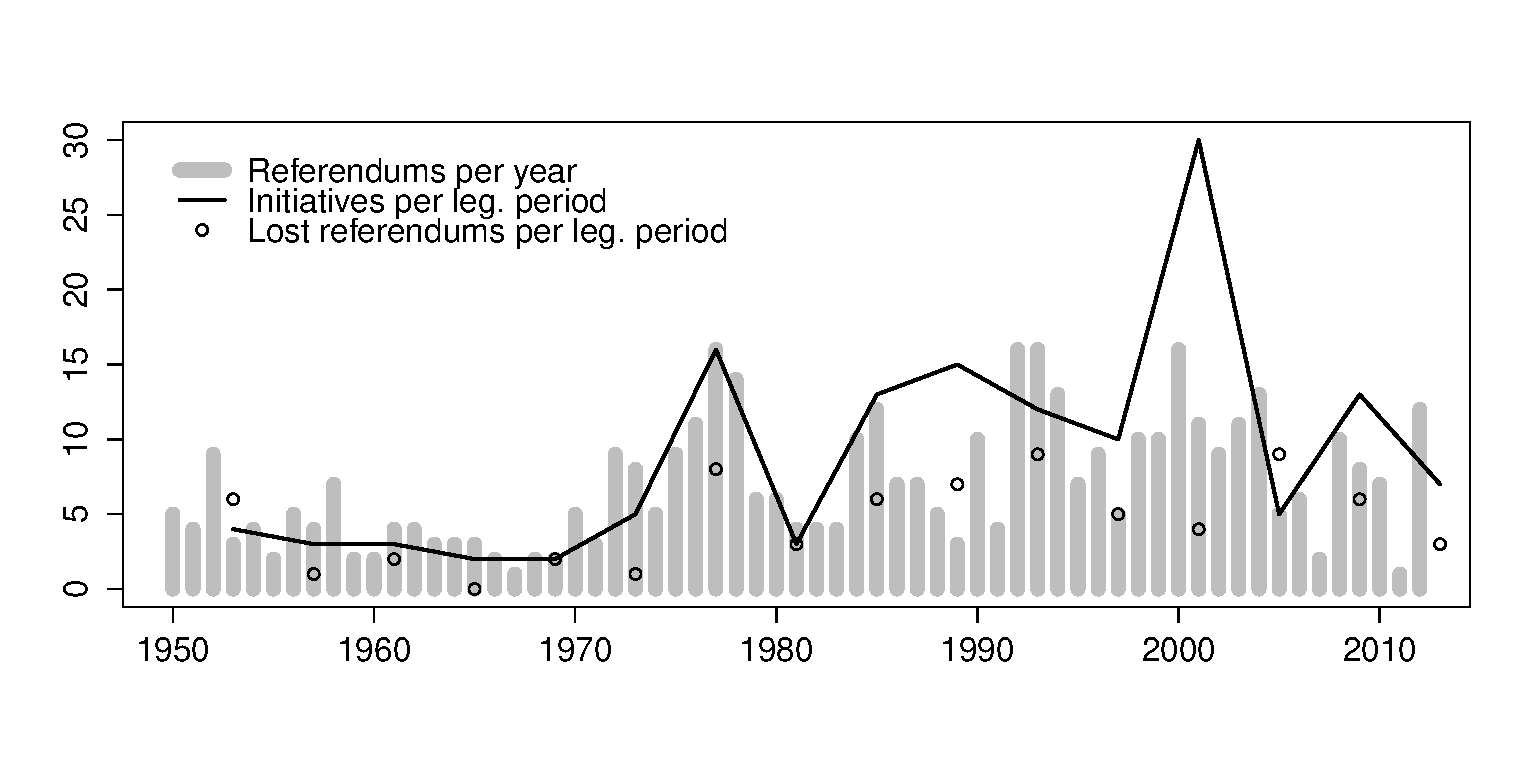
\includegraphics[width=\textwidth]{../../figures/figure.pdf}
\centering
\begin{knitrout}
\definecolor{shadecolor}{rgb}{0.969, 0.969, 0.969}\color{fgcolor}

{\centering 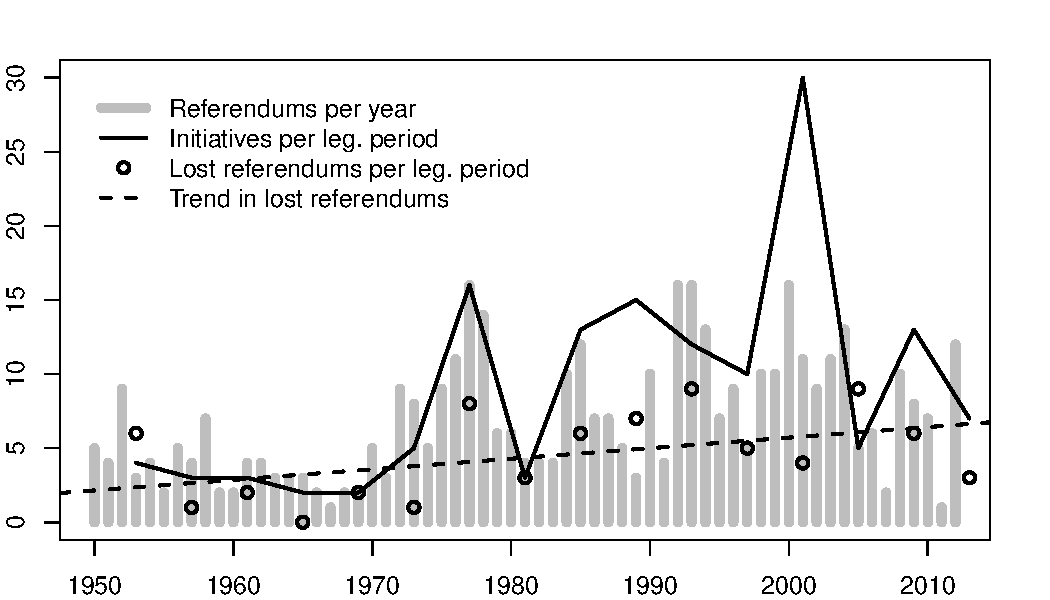
\includegraphics[width=\maxwidth]{figure/fig1-1} 

}



\end{knitrout}
\caption{Number of national referendums, initiatives and referendums lost by the government in Switzerland (1950-2013). Counts per legislative period plotted at midpoint of legislative period.}\label{fig}
\end{figure}

\section{Studying referendum voting}\label{sec:litreview}

    The literature on political behavior is immense and its subfield voting behavior is rife with highly specialized sub-topics. Yet, notwithstanding its breadth by and large the latter is a literature of electoral behavior. For instance, the Oxford Handbook of Political Behavior \citep{dalton_oxford_2007} contains no article on referendums. 
	
    There are both substantive and practical reasons why referendums have received little attention in the voting literature. Substantively, referendums have been of great appeal to theorists as embodiment of democracy, yet because of their lack of prominence in actual politics referendums have been of lesser interest to scholars of voting behavior. However, this is changing. 
    As the usage and institutionalization of referendums has increased all around the world, so has academic interest in it. It is most prominent in Switzerland and the US. In the latter which is the origin and focus of much of the recent work on direct democracy new states are adopting it at a rate of one state per decade while there has been a rise in the number of initiatives in the past decades \citep{matsusaka_direct_2005}. The number of national referendums held in Switzerland has also increased steadily since the 1950s – with peaks of usage in the 1970s and 1990s. The pattern is similar to that in the EU \citep{leininger_direct_2015}. Beyond the US and Switzerland the number of countries providing mechanisms of direct democracy has increased as has the usage of those mechanisms in all parts of the world. Among 58 democracies with a population above 3 million in the world 39 have conducted at least one referendum between 1975 and 2000 \citep[29]{altman_direct_2010}. %As referendums enjoy a more important role in politics, academic interest in them has increased.
		
    A practical explanation for the dearth of studies is simply data availability. As referendums occur infrequently and most often on the subnational level not many scientific surveys exist that would allow political scientists to investigate voting behavior in referendums. While practically all national and many subnational elections are accompanied by scientific surveys making political behavior a ``data-rich'' \citep[4]{dalton_citizens_2007} field of research this does not extend to referendum voting. 
	
	For this reason much research has been at the aggregate level, relating referendum outcomes to other macro level factors -- either across different referendums or across voting districts within a referendum. Studies that focus on the individual level are rarer and tend to focus on single referendums for which survey data happens to be available. % examples
    Even more scarce are comparative studies of referendum voting that focus on more than a single referendum -- be it multiple referendums within a country or referendums across a number of countries.
    
    Referendums differ markedly across time and space in topic and type\footnote{For typologies of direct democratic institutions interested readers are referred to \citep{altman_direct_2010} and \citep{hug_occurrence_2004}.} While elections at a given level of government within one country are relatively constant with regards to the electoral system and party system this is not the case for referendums. The institutions of direct democracy are relatively stable just as electoral systems, however no referendum vote is like another as the topic  of a vote is always a different and new one.
    
    This necessitates having a framework which allows comparative work that transcends individual referendums. One such framework is the study of EU referendums. Fifteen of now 28 member states (eight of ten that joined in 2014) have decided on their accession to the EU by means of a national referendum. A number of studies have analyzed these votes. However, they have been more interested in attitudes towards the EU seeing the referendums as an opportunity to study citizens' attitudes rather than being interested in referendums per se.
    
    It is my contention that comparative studies of referendums profit from abstracting away from topics. A small number of approaches that satisfy this criterion exist. The most prominent strand of this literature is on information in referendum voting.
    
    On election day citizens in polities with the referendum are not just confronted with a number of representatives to elect but also a number of ballot propositions. This puts high cognitive demand on voters who might not possess the information necessary to make an informed decision. 
    
    However, a number of studies find that voters can use cues from parties or interest groups to reach the decisions they would have taken had they had more information (Lupia, 1994). For Switzerland, \citet{christin_interests_2002} show that uniformed voters who received voting cues are able to vote similarly to informed voters. This literature often involves the use of interaction terms to compare the whether the effect of other covariates is different or similar for informed and uninformed voters who receive cues. 
    There also is a related literature on consistent vote choices and ambivalence in referendum voting. \citet{lanz_vote_2014} find that voters are more likely vote consistent with their argument-based opinion when referendum campaigns are intense, whereas  \citet{nai_cadillac_2014} focuses on ambivalence He finds more intense campaigns to be associated with greater voter ambivalence, that is believe in both pro- and con-arguments on a ballot proposal.
    
    Relatedly, voters, particularly, uninformed voters who received no cues, tend to display status quo bias. As voters are risk-averse they tend to stick to what they know. Voters are familiar with the status quo, which can be a policy or candidate, and need to be convinced of the alternative, challenger or new policy -- this also holds for Swiss referendums \citep{brunetti_status_1997}. %Passy (1993: 223–227) provides evidence that less-well informed voters are more likely to vote against a ballot measure and that these votes decided the referendum in at least two cases. 
    \citet{buri_grunde_1993} and \citet{christin_interests_2002} report similar results. 
    %elections referendum on incumbent performance % cite Hibbs?
    
    It is tempting to simply apply the standard Michigan model with its three interrelated factors party identification issue and candidate orientation to referendum voting. However, there obviously are no parties or candidates to elect but only an issue to decide in a referendum. In some referendums ``[v]oters must choose among alternatives that are sometimes unfamiliar and perhaps lacking in reliable voting cues'' while at other times referendums can be ``highly partisan contests, even without the appearance of party or candidate names on the ballot'' \citep[711]{leduc_opinion_2002}. 
    
    \citet{schoen_wahlen_2012}, for instance, cautions that while determinants of participation in elections and referendums are similar, determinants of vote choices differ drastically between elections and referendums. He argues that referendums, particularly initiatives, are used for proposals that found no majority or were not sufficiently addressed in the representative system. They can also be used by representatives to `outsource' contentious issues to the electorate. When this is the case, other societal actors become more prominent. \citet{schoen_wahlen_2012} illustrates this with a 2010 referendum in Bavaria, a federal state of Germany. In the referendum voters voted on a citizens' initiative that demanded that strict non-smoker protection legislation. The referendum campaign was dominated by two interest groups specially created for the purpose of campaigning for and against the initiatives's proposal. Bavaria's main political parties and their leaders did not involve themselves heavily in the campaign. This resulted in a low-key referendum campaign that was dominated by political actors outside of usual political cleavages. 
    
    \citet{clarke_referendum_2004} articulate an opposing standpoint. In a follow-up to an analysis of voting behavior in the 1995 referendum on Quebec sovereignty by \citet{nadeau_attitude_1999} they find party identification and feelings toward party leaders and government performance to be strong significant predictors of voting. They argue that in high stakes referendums where parties clearly communicate their positions standard predictors of voting behavior work well in explaining voting behavior.

    %While referendums in requiring a choice on individual issues, which might escape established party cleavages, are clearly different to elections which require a choice among multiple parties it is not clear what this means for voting behavior. 
    Whether regularities in electoral behavior can be expected to appear in referendum voting seems to be highly context dependent as the above two examples illustrate. This even holds for strong determinants like party identification. If parties refrain from campaigning on a referendum as in the example of the Bavarian referendum, party identification will play a much lesser role in determining vote choice. However, if they play an active role as in the 1995 referendum in Canada, traditional predictors can be quite relevant. What factors are important cannot (yet) be theoretically deduced but needs to established empirically.

    \section{Voting against the government}\label{sec:voteagainst} %'Voting against the government' as framework for comparative analysis of referendum votes
    
    While the previous section has highlighted some of the problems associated with analyzing referendums in a comparative framework, referendums are not necessarily more difficult to put into an analytical framework amenable to a comparative and cumulative research agenda than are elections. Voting research has become a broad and cumulative field of research by focusing on aspects such as voting for or against the incumbent, for or against right-wing parties or ticket-splitting that are common to many elections. 
    
    Referendums, too, can be systematically analyzed using such abstractions For instance, referendums on similar topics haven been successfully analyzed in a comparative fashion, e.g. EU integration \citep{hobolt_when_2005}. In Switzerland research has focused on votes on foreign and immigration policy \citep{sciarini_two-level_2009,sciarini_campaign_2011} and environmental topics \citep{bornstein_voting_2008}. However, this limits the analysis to a small number of comparable referendums. Also, such studies do not provide the possibility to discern whether correlations are idiosyncrasies of a topic or systematic features of referendum voting.

    Here, I define an outcome variable that is consistent across practically all Swiss national referendums. This variable captures whether voters voted contrary to the government issued vote recommendation. This outcome is of normative interest as direct democracy has been criticized for being an institution allegedly directed against the representative process -- a `tool for populists'. Thus, it is interesting to understand what makes voters turn against the government in a referendum vote. This paper is in part motivated by the observation of a recent increase in referendums lost by the government in Switzerland.
    
    A drawback of such an outcome measure is of course that it requires a government vote recommendation. Referendums where the government remains neutral cannot be analyzed. Or, one has to find other ways to identify a government position.
    
    As \citet{schoen_wahlen_2012} warns, determinants of participation are very similar for elections and direct democratic votes, however they can be very different for the choices made in those votes. Lacking strong theoretical expectations to inform development of hypothesis I chose a more probing approach. The following presents a number of possibly relevant correlates in the form of directed questions.
    
    My approach is descriptive in nature. I focus on identifying determinants of the above defined outcomes rather than precisely estimating a specific determinant. The partial correlations presented in section \ref{sec:results} should thus not be treated as causal \citep{keele_perils_2014}. For instance, the inclusion of political knowledge in the regression models is motivated by the normatively and politically important question whether voters who vote contrary to the government's recommendation are less well informed than other voters - holding some, not necessarily all relevant, covariates constant. It is not motivated by the question whether the lack of knowledge causes voting against the government.
    
    % Überleitung 
    
    \textbf{Age} is included in the model because one can expect that as citizens get older they become more likely to support the status quo. In the case of initiatives this implies opposing the initiative as it seeks to change the status quo. Here, rejection of change would lead to a vote for the government position. However, obligatory and facultative referendums are votes on government initiated changes to the status quo. In that case, if older voters are indeed more risk averse they should then should be more likely to vote against the government. Yet, older citizens also tend to be more trusting in government. This leads to the following question.
    
     \begin{question}
      \begin{minipage}[t]{4 in}
    	Are older citizens more likely to support the government's position than younger citizens?
      \end{minipage}
     \end{question}
    
    Expectations are less clear for the role of \textbf{gender} in referendum voting.  However, it is well established that there is a significant gender gap in support for right-wing parties. Men are much more likely to support such parties. Relating this to the populist notion of voting against the government and sometimes populist or even right-wing nature of initiatives one could expect men to be more likely to vote against the government. Switzerland, although a long-established democracy, introduced women's suffrage extremely late - by referendum in 1971. Still, only a third of the members of the Swiss parliament's lower house (German: \textit{Nationalrat}, French: \textit{Conseil National}) are women. Possibly this puts women into opposition to male-dominated politics in referendums. This motivates the following question.
    
    \begin{question}
      \begin{minipage}[t]{4 in}
	    Are male voters more likely to vote against the government than female voters?
      \end{minipage}
    \end{question}
    
    %\textbf{Q} Interaction effect between age and type
    
    People with higher levels of \textbf{education} should be more confident about their ability to participate in referendums \citep{collingwood_levels_2012}. 
    As regards the normatively and empirically controversial questions of minority rights under direct democracy highly educated voters are said to be more likely to support minority rights \citep{bowler_demanding_1998,anderson_why_2010}. \citep{vatter_who_2014} shows this to be the case in Swiss referendums, too, this topic appears on the ballot quite frequently. Infringements of minority rights via the initiative are usually opposed by the government. Also highly educated citizens should also be less prone to support populist initiatives. This brings up the following question. 
    
     \begin{question}
     	\begin{minipage}[t]{4 in}
    	Are highly educated voters less likely to vote against the government?
    	\end{minipage}
     \end{question}
    
    
    As regards \textbf{political knowledge} I focus on voters' referendum-specific knowledge. \citet{christin_interests_2002} find a negative relationship between political knowledge and voting against the status quo. Again a status quo bias argument can be made that would suggest that uninformed voters are more likely to vote against the government on counter-proposals, obligatory and facultative referendums but not initiatives. Interestingly, half of the referendums studied by \citet{christin_interests_2002} where this relationship does not hold are initiatives. Yet, they caution against interpreting this to mean that uninformed voters vote against the government. This motivates the following question.       
    
     \begin{question}
      \begin{minipage}[t]{4 in}
    	Are voters who are more knowledgeable about a ballot proposal less likely to vote against it?
      \end{minipage}
    \end{question}
    
%     the unemployed might be more disaffected and willing to use referendum as vehicle to voice their discontent. This is why I include \textbf{employment status} in the analysis. employed profit from status quo. status quo bias. mixed signal.
%     
%     \begin{question}
% 	    \begin{minipage}[t]{4 in}
% 		    Are unemployed voters more likely to vote counter a government vote recommendation?
% 	    \end{minipage}
%     \end{question}
    
    Switzerland is a multilingual nation made up of a German-speaking, a French (\textit{Romandie}) and an Italian (\textit{Italian Switzerland}) part. %The German part comprises over half of Switzerland, central, north and western Switzerland. The french-speaking part is situated in the East and is home to about a quarter of the Swiss population. Italian Switzerland comprises of south-eastern Switzerland and is the smallest of the linguistic regions. 
    These regions define cultural and political differences. The cultural and political divisions, particularly between the German and French part, are mockingly referred to as \textit{Röstigraben}, alluding to a classic Swiss-German potato dish. Indeed referendum returns often differ notably between these regions with the French part being more positive towards international openness, social policy and regulation. For instance in the recent 2014 referendum vote on curbing migration the yes-share was noticeably higher in Swiss German cantons than in the \textit{Romandie} or \textit{Italian Switzerland}. This prompts the following question. 
    
    \begin{question}
	    \begin{minipage}[t]{4 in}
	        Are French- and Italian-speaking Swiss citizens less likely to vote counter to a government recommendation?
	    \end{minipage}
    \end{question} 
    
    At the macro-level I consider, firstly, the \textbf{type} of referendum. This is for one motivated by the observation of differences in the number of government losses between types. While voters have rejected half of the counter-proposals put forward by the government they have only rejected the government policy in a quarter of obligatory and facultative referendums and rejected fully 90\% of initiatives (cf. Table \ref{tab:wonlost}). A correlation with individual-level voting behavior can, again, be motivated by status quo bias. Voting against a government proposal in an initiative means rejecting the status quo, while rejecting the government position in a vote on an obligatory or facultative referendum or counter-proposal means affirming the status quo. The former is much more demanding. This should lead one to expect a lower propensity to vote against the government for initiatives. 
    Also initiatives are not necessarily always meant to pass. Sometimes, some would say increasingly, initiatives are used by parties to campaign on their platforms and gain publicity. Sponsors of initiatives are more likely to put hard-to-win proposals on the ballot than the government. %The government will only trigger a obligatory referendum if it thinks that the proposed changes can obtain a popular majority. 
    Yet, as has been shown in section \ref{sec:introduction}, the increase in government losses has gone hand in hand with an increase in initiatives. This suggests the following question.
    
     \begin{question}
    	\begin{minipage}[t]{4 in}
    		Are voters less likely to vote against the government position on an initiative than in other referendums?
    	\end{minipage}
     \end{question}
     
%    \textbf{topic}
%    \begin{question}
%	    \begin{minipage}[t]{4 in}
%	    	Are voters more likely to reject government recommendation on matters of integration?
%	    \end{minipage}
%    \end{question} 
    	
    The literature on voting heuristics in referendums suggests that even if voters are not particularly well-informed on the subject matter of a referendum they can still cast an informed vote by relying on messages from parties and other political actors that they trust \citep{lupia_shortcuts_1994}.   
    Voters with a party identification are expected to follow their respective party's vote recommendation. Even voters who do not identify with any of the parties could be influenced if all governing parties recommend a certain position. A similar 
    %Kriesi (1994: 67) suggests that only 6 per cent of the voters are close to a politi-
    % cal party, know its endorsement and state that this endorsement was the most
    % important viewpoint influencing their voting decision.
    idea can be found in in a paper by \citet{sciarini_campaign_2011}, although they distinguish between grand, center-left and center-right coalitions. However, while \citet[766]{christin_interests_2002} conclude that ``endorsements as cues are clearly visible in Swiss referendum campaigns'', only 30\% of respondents seem to know endorsements of their party \citep{gruner_stimmburger_1983}. This leads to the following question. 
    	
     \begin{question}
    	\begin{minipage}[t]{4 in}
    	Are voters less likely to vote against a government recommendation when the governing parties are united in their vote recommendations?
      \end{minipage}
     \end{question}
    
    % another idea. per referendum: average complexity of the proposal as reported by respondents.
    
    % yet another idea. per referendum: average informedness of voters as proxy for quality of (information) campaigns. Does better information reduce likelihood of voting against government position?
    
    \section{Data \& Empirics}\label{sec:data}
    
    The data I use to address these questions are a cumulation of the \textit{VOX} post-referendum surveys, called \textit{VoxIt}, that cover 245 national referendums held in Switzerland between 1981 and 2010 \citep{brunner_voxit:_????}. These surveys contain information on respondents’ voting behavior, their personal characteristics as well as referendum-specific information.
    
    Initially there are a total of 243,214 observations, when removing respondents who did not vote or cast an empty ballot the dataset reduces to 136,537 
    observations.\footnote{I recognize that one could argue that voting in a referendum entails two choices -- whether to participate or not and how to vote if one participates -- and that both choices should be modeled. This would call for a selection model which explicitly models participation. Indeed, at the aggregate level abstention of potential backers of government policy might influence results. However, there are no theoretical reasons to think that potential backers of the government are less likely to participate than those who would vote against the government. Also, I have no theoretical arguments why the exclusion of non-voters should bias the results. Even further, the interest here is in understanding voters' decision to vote counter to the government recommendation. This is much less speculative than musing about the hypothetical voting behavior of non-voters.} Removing data on a 1996 referendum on a change to the labor law for which the government issued no vote recommendation reduces the sample size by another 577 observations. The average sample size per survey is 555 ($s$: 126). Missing answers on some independent variables reduce the sample size further (see Table \ref{tab:regtable}).
    
    Observations are clustered into referendums, referred to as \textit{projets} in \textit{VoxIt}, and a referendum day -- referred to as \textit{scrutin}. Voters may vote on multiple referendums on referendum day. My data contain 245 \textit{projets} clustered into 85 \textit{scrutins}. The number of ballot proposals on a given referendum day ranges from 1 to 6 \textit{projets} per \textit{scrutin}. The average number of referendums is 2.9 referendums per \textit{scrutin}, with the median at 3. Of these 245 referendums 98 are initiatives, 71 are referendums, 60 are obligatory referendums, while 16 are governmental counter-proposals to initiatives (cf. Figure \ref{fig:typetopic}).
    
    \begin{figure}
\begin{knitrout}
\definecolor{shadecolor}{rgb}{0.969, 0.969, 0.969}\color{fgcolor}
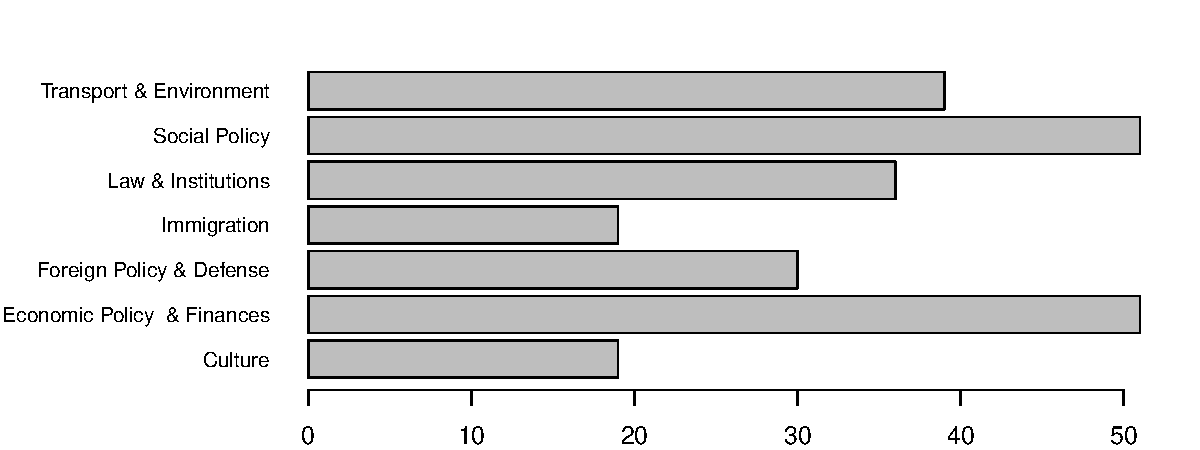
\includegraphics[width=\maxwidth]{figure/fig2-1} 

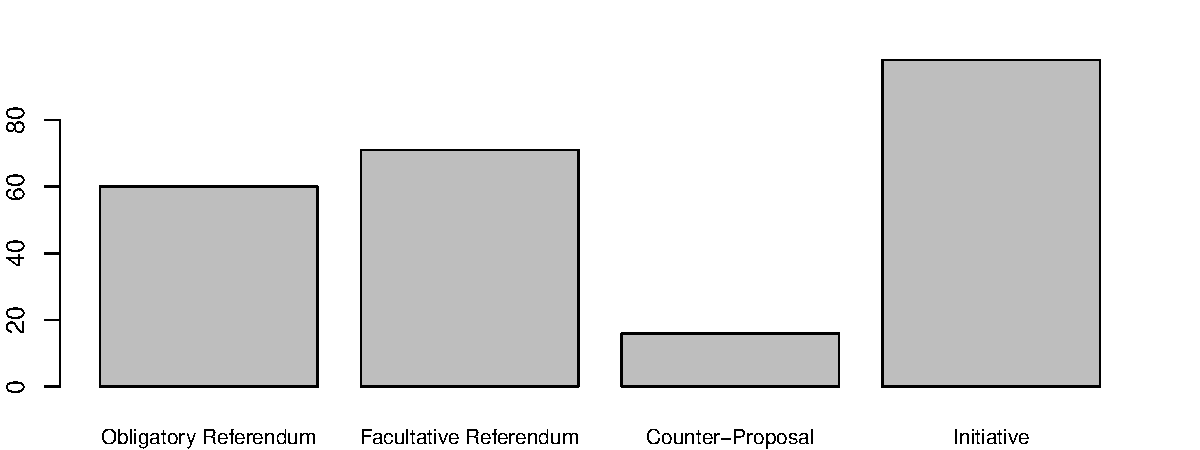
\includegraphics[width=\maxwidth]{figure/fig2-2} 

\end{knitrout}
        \caption{Number of referendums per type and topic.}\label{fig:typetopic}
    \end{figure}
    
    There is one survey, representative at the national level, per \textit{scrutin}. It is important to note that one observation is not equivalent to a unique respondent. Respondents are asked about each referendum (ballot proposal) put to a vote on referendum day. The survey data are cumulated by referendum so that any single respondent appears multiple times. The number of appearances of any individual respondent is equal to the number of \textit{projets} he or she reports her vote choice on. 
    
    Thus, the data are cross-classified as neither respondents are hierarchically sorted into referendums, nor are referendums hierarchically sorted into respondents. I consequently use a cross-classified random intercept model with random intercepts for referendums (\textit{projet}) and respondents (\textit{id}). 
	
	Random-effects models, often referred to as multi-level models, are now increasingly common in political science in general, and comparative survey research in particular. Multilevel level models have been applied to Swiss referendums a number of times \citep[e.g.][]{sciarini_two-level_2009,sciarini_campaign_2011,vatter_who_2014,lanz_vote_2014}. 
	
	Prior comparative studies of political behavior have also relied on two other approaches. Some have estimated separate regressions \citep[e.g.][]{lutz_low_2007}, others have analyzed the data in one model, including dummies for the units of the contextual level 
    \citep[e.g.][]{eichenberg_europeans_1993}. The former approach is impractical for this paper as it would necessitate the estimation of 245 separate regressions, one for each referendum. Also, results would be difficult to summarize in a convenient and understandable form for readers. The dummy variable approach effectively captures variance between higher-level units and focuses individual-level predictors on within referendum-variance. However, this precludes the estimation of context-level correlations. As I am interested in both individual-level and contextual correlations I estimate cross-classified logistic multi-level models. 
    
    Of the individual-level variables in the models two are binary variables. These are \textbf{gender} (1 = female) and another dummy capturing whether respondents hold a \textbf{university degree}. Unfortunately, respondents were not asked how many years they spend in education but they were asked to indicate their highest educational degree. This ordinal measurement (6 categories) is simplified to the above mentioned dummy -- an operationalization of education commonly used in the related literature \citep[5]{vatter_who_2014}. 
    
    \textbf{Referendum specific knowledge} is a three-categories ordinal measure based on questions asking voters about the title and content of a ballot proposal. Respondents score one if they know the title or content of a ballot proposal, two if they can name both and zero if they know neither. Scores one and two are implemented as dummies with zero as base category. The continuous predictor \textit{age} enters as z-standardized variable into the model.  
    
    %\textbf{party identification with governing party} dummy indicating whether the respondent identifies with one of the four (five after 2008) parties making up the Bundesrat. Coding of variable takes into account that the newly founded BDP has a member in federal council since 2008.
    
    For the aggregate level the \textbf{type of referendum} is captured by separate dummies for facultative referendums, counter-proposals and of course the initiative. Obligatory referendums serve as base category.
    \textbf{Governing party unity} captures how united the governing parties are in backing the official government position. As the Bundesrat consisted of four parties until 2008 and five parties thereafter the variable is coded as proportion of governing parties that recommend the government position.
    
    %\textit{topic} VOX data classified referendums into length(levels(d$themex)) different categories. Narrowed this down to length(levels(d$topic)) topics to make tractable for analysis.
    
    %As in most studies there is overreporting of turnout. Is there underreporting of against the government votes?
    
    Lastly, a technical note: the data have been prepared and analyzed using the statistical software package \texttt{R} \citep{r_core_team_r:_2014}, using the package \texttt{lme4} \citep{bates_lme4:_2014} for multilevel models. The code used to produce the tables and figures in this paper (available on \textbf{GitHub}) is embedded into the source code using \texttt{knitr} \citep{xie_knitr:_2014}.
    
    \section{Results}\label{sec:results}
    I estimated cross-classified multilevel models to obtain correlations between voting against the government and both individual and referendum-specific factors. The goal of this descriptive exercise was to identify potential determinants of the above defined outcomes rather than precisely estimating a specific determinant. Estimates obtained from such a regression analysis should not be treated as causal -- see for instance \citet{keele_perils_2014} for a persuasive exposition. Consequently, I use the word `partial correlation' or equivalents when referring to coefficient estimates and refrain from using the word `effect.' The rudimentary analysis presented here (cf. Table \ref{tab:regtable} and Figure \ref{fig:coef}) provides an initial yes-answer to five of the seven questions posed in section \ref{sec:voteagainst}.
    
    All coefficients, except for counter-proposals and initiatives, are significant at the 5\% level or higher. P-values were obtained through Wald tests ($\frac{\beta}{se}$). These rely on asymptotic theory, implying that as the highest level unit size approaches infinity, such tests will be normally distributed. Although the number of level-2 units (\textit{projet} and \textit{id}) is very high compared to usual sample sizes in comparative survey research, results should be taken with a pinch of salt.\footnote{Alternatives are using bootstrapping or Bayesian estimation both of which require extensive and time-consuming are computations. They will be considered for future revisions.} %This is only a first rudimentary look at the data. 
    
    \begin{figure}[htb]
\begin{knitrout}
\definecolor{shadecolor}{rgb}{0.969, 0.969, 0.969}\color{fgcolor}
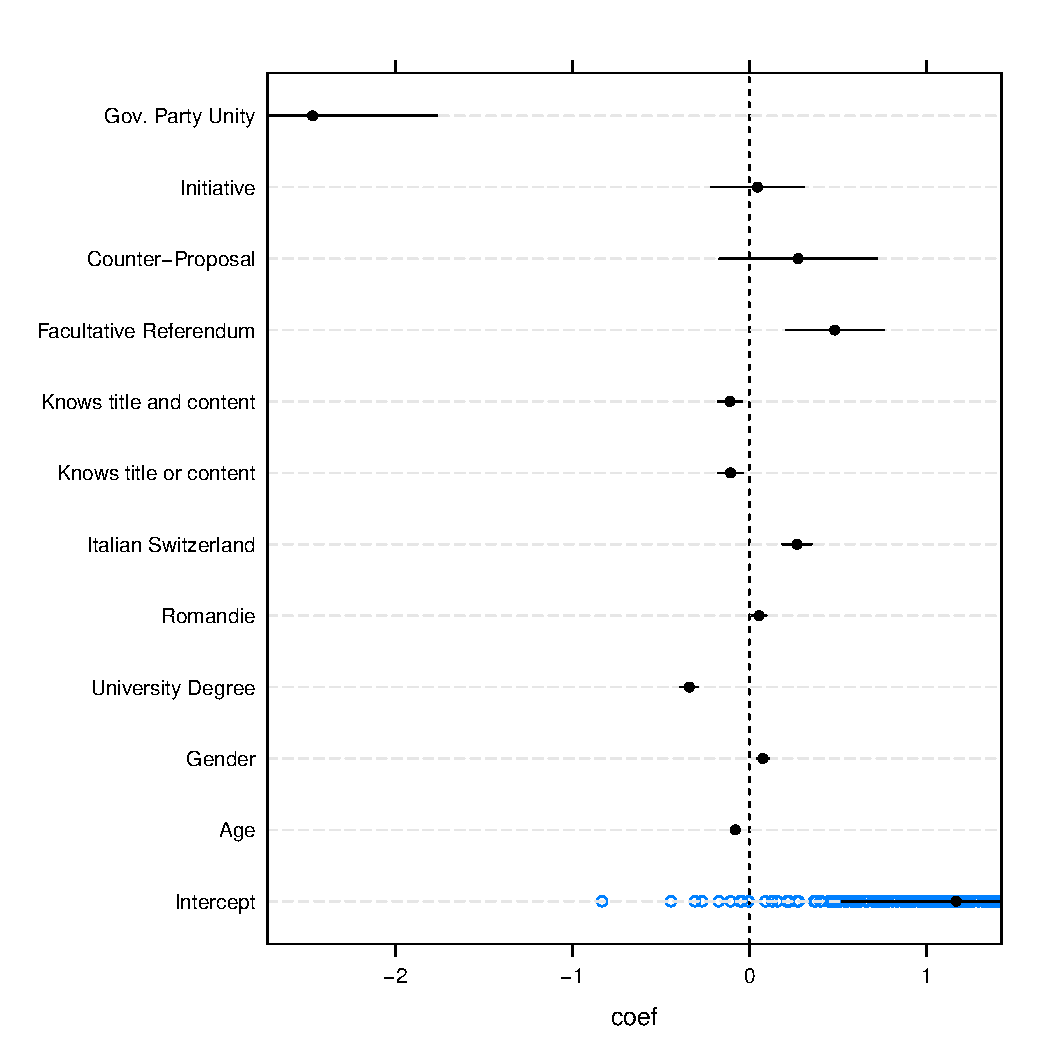
\includegraphics[width=\maxwidth]{figure/fig3-1} 

\end{knitrout}
        \caption{Dots are unstandardized coefficient estimates, lines are 95\% confidence intervals and hollow circles are empirical Bayes predictions of the random intercept (\textit{projet}).}\label{fig:coef}
    \end{figure}
    
    The coefficient on age is negative suggesting that older respondents, when controlling for the other covariates, are less likely to vote against the government. There are two interpretations to this finding. Either, respondents become more supportive of government policy as they get older. Or, the partial correlations indicate a generational difference. Possibly, younger generations grew up to be more critical of authorities and government, therefore more likely to reject the government position. %and do not necessarily that the propensity of individuals to vote against the government changes as they age. 
    This has different implications for understanding trends at the aggregate level as I discuss in the next section.
    %  If this is a generation effect than this woul imply a trend in rejection of government proposal. As citizenry becomes more critical likelihood of rejection increases.
    
    The preliminary answer to the question whether men are more likely than women to vote counter to a governmental vote recommendation is no. There is no quick explanation for this pattern. If anything, the literature on populist parties would lead one to expect a different relationship. Citizens with a university degree are indeed less likely to vote against the government. However, again, one should not hastily interpret this as an educational effect. 
    
    Contrary to what the question about regional identity implied voters from the \textit{Romandie} and \textit{Italian Switzerland} are more likely to vote against the government than \textit{Swiss-German} voters. The question has been guided by the popular perception that Swiss Germans more likely to support restrictives initiatives such as the February 2014 anti-immigration initiative. It would be interesting to look at what the referendums were on which French- and Italian-Swiss voters voted more frequently against the government than Swiss Germans.
    
     \begin{table}[htb]
    \centering\footnotesize

\begin{tabular}{l D{.}{.}{6.5}@{} D{.}{.}{6.5}@{} D{.}{.}{6.5}@{} }
\toprule
                              & \multicolumn{1}{c}{ID} & \multicolumn{1}{c}{Projet} & \multicolumn{1}{c}{Full model} \\
\midrule
ID                            &            &             &             \\
                              &            &             &             \\
\quad Age                     & -.08^{***} &             & -.08^{***}  \\
                              & (.01)      &             & (.01)       \\
\quad Gender (1=female)       & .08^{***}  &             & .08^{***}   \\
                              & (.02)      &             & (.02)       \\
\quad University degree       & -.34^{***} &             & -.34^{***}  \\
                              & (.03)      &             & (.03)       \\
\quad Romandie                & .06^{**}   &             & .06^{**}    \\
                              & (.02)      &             & (.02)       \\
\quad Italian Switzerland     & .27^{***}  &             & .27^{***}   \\
                              & (.04)      &             & (.04)       \\
\quad Knows title or content  & -.10^{**}  &             & -.11^{**}   \\
                              & (.03)      &             & (.03)       \\
\quad Knows title and content & -.11^{**}  &             & -.11^{**}   \\
                              & (.03)      &             & (.03)       \\
Projet                        &            &             &             \\
                              &            &             &             \\
\quad Facultative Referendum  &            & .46^{***}   & .48^{***}   \\
                              &            & (.13)       & (.14)       \\
\quad Counter-Proposal        &            & .28         & .28         \\
                              &            & (.21)       & (.23)       \\
\quad Initiative              &            & .05         & .05         \\
                              &            & (.12)       & (.13)       \\
\quad Gov. Party Unity        &            & -2.46^{***} & -2.47^{***} \\
                              &            & (.28)       & (.36)       \\
Intercept                     & -.62^{***} & 1.08^{***}  & 1.17^{***}  \\
                              & (.07)      & (.25)       & (.33)       \\
\midrule
AIC                           & 148274.88  & 151129.15   & 148217.73   \\
BIC                           & 148372.21  & 151197.40   & 148353.99   \\
Log Likelihood                & -74127.44  & -75557.58   & -74094.86   \\
Num. obs.                     & 124576     & 126688      & 124576      \\
Num. groups: id               & 46226      & 47294       & 46226       \\
Num. groups: projetx          & 244        & 245         & 244         \\
Variance: id.(Intercept)      & 1.03       & 1.04        & 1.03        \\
Variance: projetx.(Intercept) & .78        & .60         & .60         \\
Variance: Residual            & 1.00       & 1.00        & 1.00        \\
\bottomrule
\multicolumn{4}{l}{\scriptsize{$^{***}p<0.001$, $^{**}p<0.01$, $^*p<0.05$}}
\end{tabular}

    \caption{Cross-classified random-effects model with binary indicator for vote against government as dependent variable. Unstandardized regression coefficients.}\label{tab:regtable}
    \end{table}
    
    The two dummy variables for referendum specific knowledge carry negative coefficients. More knowledgeable respondents are less likely to vote no. Yet, there is no great difference between those who know the title or content of a ballot proposal and those that know both. This is not to say that raising levels of information will decrease anti-government voting, however it is an interesting initial finding. As mentioned numerous times before, less knowledgeable voters are more prone to status quo bias. As the status quo varies by referendum this would be one obvious possible interaction term to include in further models: $knowledge \times type$. There surely are more theoretically relevant interactions. 
    
    Voters are more likely to vote no on facultative referendums. This finding matches the aggregate numbers where 21 (27.6\%) facultative referendums have been lost by the government, second only to counter-proposals. However, there have only been 18 counter-proposals between 1981 and 2010.
    
    Finally, when the governing parties are united in recommending the official government position voters are less likely vote against it. One possible reason is that such unity sends a strong message to voters. However, this would need to be corroborated in further analyses. The present finding could also simply reflect that on uncontroversial government policies and fringe initiatives there is a broad consensus among citizens and elites -- which for the former would also exist in absence of voting recommendation issued by the parties. 
    
    \section{Discussion}\label{sec:discussion}
    
    % shortcomings: only Swiss data
    
    Taking note of an upward trend in the number of referendums the government loses I proposed to study the correlates of voting against the government. Such a framework allows for the comparative analysis of the complete set of Swiss national referendums for which survey data is available. It is also applicable to other countries where such governmental vote recommendations exist or the government's position on a referendum can be credibly established through other means. In principle it also allows the study of referendums across borders. 
    
    An initial exploratory analysis has identified a number of interesting correlates that merit further analysis. Obviously such a rudimentary analysis has several shortcomings, one of them being the omission of other relevant variables. %In this preliminary analysis I was only able to consider a small number of predictors. modification of existing variables
    These comprise for instance knowledge of the government's vote recommendation. Is voting against the government correlated with a lack of knowledge of the government's position? Also, it seems particularly relevant to include the voters' assessment of the likely impact of the proposal on the respondent him- or herself or the nation in general. These can be important predictors for high-stakes referendums \citep{nadeau_attitude_1999}. The analysis as of yet omits classic predictors like party identification or left-right self-placement. These are not straightforward to incorporate. Including the latter poses problems because the self-placement question was changed at least once during the time period studied. Party identification could be summarized in one variable indicating whether the respondent identifies with one of the four (five after 2008) parties making up the Bundesrat. Combining party identification with the parties' recommendations would allow investigating the effectiveness of such cues. 
    % trust in government or modus of voting: ballot, Stellvertreter, postal or online.
    
    %the unemployed might be more disaffected and willing to use referendum as vehicle to voice their discontent. This is why I include \textbf{employment status} in the analysis. employed profit from status quo. status quo bias. mixed signal.
    
    %as well as the campaign waged by proponents and opponents in the lead-up to a referendum.
    Of particular relevance to parties and governments, lastly, is the question whether campaigns can encourage citizens to vote in the desired way. Measuring campaigns is a tricky issue and aggregate data is hard to come by or laborious to collect. One remarkable effort is Nai's \citeyear{nai_choisir_2013} dataset on 75 campaigns between 1999 and 2005 based on an analysis of campaign ads in Switzerland's major newspaper. For a study of the full cumulation of referendums the mean referendum specific knowledge of voters per referendum could be used as proxy for the reach of the campaigns. Does better information reduce the likelihood of voting against the government?
    
    The time span the survey data cover is substantial -- 32 years from 1981 to 2010. Obviously many things can and do change in such a long time period. Interacting predictors with a time variable allows an assessment whether correlations have changed over time and is a possibility for future revisions.
    
    Identifying predictors for voting against the government does not necessarily reveal the motivations of such voters. It might be helpful to have not just predictors but also a typology of voters. How could one, among the voters `defying' the government, for instance, distinguish `reasoned' from `populist deviators'?  Who substantively disagrees with the government's position and who is rather motivated by expressing his or her discontent? Political knowledge seems to be of key importance here. Somebody who voted against the government and cannot provide title, content or arguments likely is not a `reasoned deviator.' %Somebody might not knowingly vote against the government but still vote against it out of his or her arguments-based opinion. It is not strictly necessary to know the government's position to be an informed deviator. To be a `populist' deviator one arguably needs to know the government's position.  %combination of knowing government position and not being well-informed.
    
%    \begin{figure}[htb]
%    bars and boxplot at the side.
%    \caption{uninformed non-voters per referendum}\label{fig:deviators}    
%    \end{figure}
    
   The increase in government losses alluded to in the introduction fits with a general story of increasing political discontent among citizens and a rise of populist parties  \citep[e.g.][]{mair_ruling_2013}. How can an analysis of individual voting behavior contribute to explaining the macro-level trend in rising numbers of government defeats? 
   This trend could be rooted in both macro and individual level factors. Given the results presented in this paper the parallel increase in initiatives does not seem to be a prime contender for a possible explanation. There is no strong evidence that voters are more likely to vote against the government's recommendation. On the individual level, a decline in party identification in the voting population could explain why voters increasingly disregard their government's vote advice. However, one would first need to establish whether these are relevant at all. If one believes that the correlation with age found in this analysis is genuine one could construe a trend from this finding. Assuming that this correlation captures a generational effect, the average likelihood for a voter to vote against the government will increase over time as older generations exit and younger generations enter the electorate. 
    
    
    \small\printbibliography

\end{document}
